\documentclass{article}
\usepackage[utf8]{inputenc}
\usepackage[spanish]{babel}
\usepackage{graphicx}
\usepackage{anysize}
\usepackage{fancyhdr} 
\usepackage[export]{adjustbox}
\usepackage{titlesec}
\usepackage{enumitem}
\usepackage{amsmath}
\usepackage{amssymb}
\usepackage{listings}
\usepackage{xcolor}
% \usepackage{hyperref}
% \usepackage{float}
% \usepackage{tabu}

% Izquierda, derecha, arriba, abajo
\marginsize{1.5cm}{2cm}{1.2cm}{1cm} 
\renewcommand{\familydefault}{\sfdefault}
\decimalpoint%

\graphicspath{{assets/}{bdd_prac_06.assets/}}

\setlength{\parindent}{0in}
\titleformat*{\section}{\large\bfseries}

% Para insert código
\definecolor{codegreen}{rgb}{0,0.6,0}
\definecolor{codegray}{rgb}{0.5,0.5,0.5}
\definecolor{codepurple}{rgb}{0.58,0,0.82}
\definecolor{backcolour}{rgb}{1,1,1}

\usepackage{textcomp}
\lstset{upquote=true}
\lstdefinestyle{mystyle}{
    backgroundcolor=\color{backcolour},   
    commentstyle=\color{codegreen},
    keywordstyle=\color{magenta},
    numberstyle=\tiny\color{codegray},
    stringstyle=\color{codepurple},
    basicstyle=\ttfamily\footnotesize,
    breakatwhitespace=false,         
    breaklines=true,                 
    captionpos=b,                    
    keepspaces=true,                 
    % numbers=left,                    
    % numbersep=5pt,                  
    showspaces=false,                
    showstringspaces=false,
    showtabs=false,                  
    tabsize=2
}

\lstset{style=mystyle}

\newcommand{\materia}{BDD}
\newcommand{\clave}{2947}
\newcommand{\profesor}{Ing. Rodriguez Campos \textsc{Jorge Alberto}}
\newcommand{\grupo}{1}
\newcommand{\semestre}{2021-1}

\newcommand{\alumno}{
    Francisco Pablo \textsc{Rodrigo}  \\ 
    Flores Martinez \textsc{Emanuel}   
}

\newcommand{\actividad}{Práctica 06}
\newcommand{\titulo}{Transparencia de distribución - Mapeos locales}

\newcommand{\fechaEntrega}{30 noviembre de 2020}

%%%%%%%%%%%%%%%%%%%% ENCABEZADO %%%%%%%%%%%%%%%%%%%%%%%%%%%%
\pagestyle{fancy}
\fancyhf{}
\renewcommand{\headrulewidth}{0pt}
\fancyhead[R]{% Left header
    \begin{tabular}{l}
        \materia \\ 
        \actividad%
    \end{tabular}
    \,% Space
    \rule[-1.75\baselineskip]{0pt}{0pt}
    % Strut to ensure a 1/4 \baselineskip between image and header rule
    
\includegraphics[height=3\baselineskip,valign=c]{unam}
}
\setlength{\headsep}{0.3in}


\begin{document}
%%%%%%%%%%%%%%%%%%% DATOS PORTADA %%%%%%%%%%%%%%%%%%%%%%%%
\thispagestyle{empty}
\begin{minipage}[t][5cm][t]{0.2\linewidth}
    
\includegraphics[width=2.5cm]{unam.jpg}
    \vspace{10cm}

    
\includegraphics[width=2.5cm]{fiblack}
\end{minipage}
\begin{minipage}[t]{0.7\linewidth}
    \vspace{-2.5cm}
    \LARGE{\textbf{Universidad Nacional Autónoma de México}}\\
    \Large{\textbf{Facultad de Ingeniería}} \\

    \large{\semestre}\\[2cm]

    \large{\textbf{\materia (\clave)}}\\
    \large{\textbf{Gpo: 1}}\\[5mm]
    \large{\textbf{Profesor:} \profesor}\\ [1.5cm]
    \begin{center}
        \LARGE{\textbf{\actividad}}\\
        \LARGE{\textbf{\titulo}}\\
    \end{center}

    \vspace{3.3cm}

    % \large{\textbf{Alumno:} \alumno} \\[1.5cm]
    \large{
        \begin{itemize}[
            noitemsep,
            % topsep=0pt,
            % parsep=0pt,
            % partopsep=0pt,
            % labelwidth=5cm,
            align=left,
            % itemindent=2cm
        ]
            \item [\textbf{Alumno(s):}] 
            \begin{flushright}
                \alumno
            \end{flushright}
        \end{itemize}
    } \vspace{1.5cm}

    \begin{flushright}
        \fechaEntrega%
    \end{flushright}
\end{minipage}

\newpage
%%%%%%%%%%%%%%%%%%% CONTENIDO %%%%%%%%%%%%%%%%%%%%%%%%

\section*{Introducción}
% TODO:- Hacer introducción en tiempo futuro

\section*{Objetivos}

Comprender la forma en la que se realiza la configuración de una base de datos 
Oracle para implementar el concepto de Transparencia de distribución en su 
primer nivel: Mapeos Locales. La implementación de este nivel se realizará a 
través del uso de PDBs y ligas (database links) para establecer una 
comunicación bidireccional.

\section*{C1. Diagrama Jerárquico }

% TODO:- Insertar imagen, una por equipo
%\lstinputlisting[language=SQL]
%{bdd_prac_05-codigo/s-04-rfp-consulta-fragmentos.sql}

\section*{C2. Investigación modo dedicado/ modo compartido }

% TODO:- Agregar investigacion

\section*{C3. Código únicamente para \texttt{suscriptor} y ejecución del 
  script \texttt{s-03-<SID>-consultas.sql}}

%\lstinputlisting[language=SQL]
%{bdd_prac_05-codigo/s-07-rfp-consulta-datos.sql}

%\textbf{Salida del script anterior}\\
%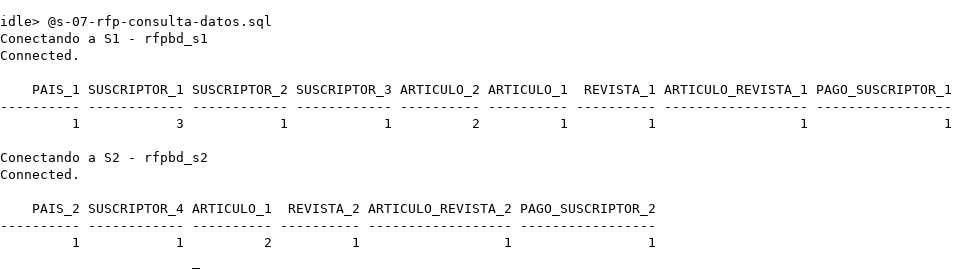
\includegraphics[width=\linewidth]{bdd_prac05-c3-consulta-datos}

\section*{C4. Actualización de fragmentos de código para el procedimiento 
  \texttt{guarda\_blob\_en\_archivo}}

 \section*{Salida de ejecución del script de validación 
  \texttt{s-05-validacion-main.sql}}
  
\section*{Comentarios y conclusiones}

% TODO:- Agregar comentarios

\renewcommand\refname{Bibliografía}
\begin{thebibliography}{99}
    \bibitem{oracle} Oracle. \textit{Oracle Database Documentation} en 
        \texttt{https://docs.oracle.com/en/database/oracle/\\oracle-database/%
        index.html}
    \bibitem{oracledb} Oracle Database. \textit{Database PL/SQL Language 
        Reference} en 
        \texttt{https://docs.oracle.com/en/database/oracle/\\
        oracle-database/12.2/lnpls/database-pl-sql-language-reference.pdf}
    %  TODO:- Add more references
\end{thebibliography}

\end{document}
